\chapter{Exercise 5}
The purpose of the exercise is to get acquainted with input and
window management in Glut and OpenGL. In particular we will
work with mouse input, keyboard input, menus, multiple windows,
logic operations, selection and picking.

\section{Part 1}
	Pick function is choosing which type of object will be drawn, basing on
	a position of a mouse.
\section{Part 2}
	Performing a selection required following steps:
	\begin{enumerate}
	\item Build a texture
	\item Bind a texture to a frame buffer object
	\item Render the scene to a FBO with ids encoded as colors
	\item When click event is called, decode a pixel color on mouse position using FBO
	\item Decoded value is an object id
	\end{enumerate}	 
\section{Part 3}
I made a program, which can draw and edit simple circuit diagrams. My sample
diagram can be seen in the figure \ref{fig:exercise_5_part_3}.
\begin{figure}[ht!]
	\begin{center}
		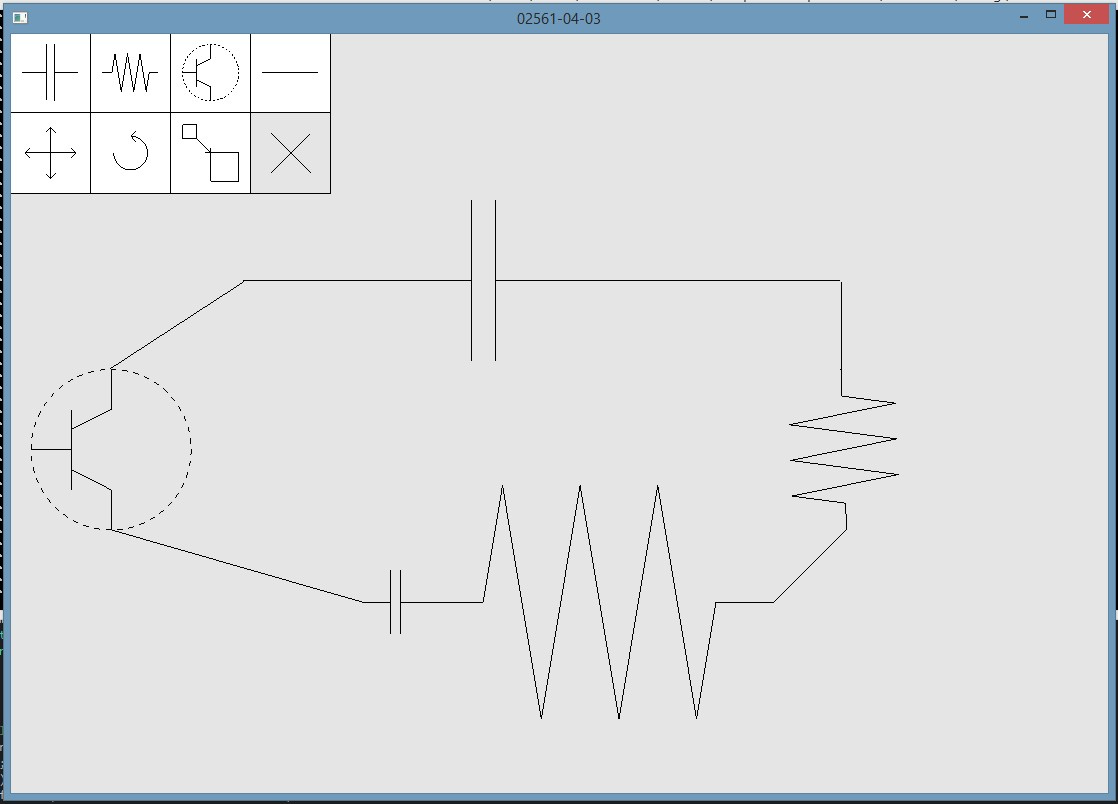
\includegraphics[width=1.0\textwidth]{figures/exercise_5_part_3}
	\end{center}
	\vspace{-4.5ex}\caption{Exercise 5 part 3 output}
	\label{fig:exercise_5_part_3} 
\end{figure}